% questions.tex —— 1977 年·河北卷 · 题目内容片段（无答案）
% 由 tools/generate_projects.py 依来源总账自 1977/1977_数学真题_河北_试题.md 生成，勿手改（改源 MD 后重跑）


\gkpart{数学试卷（河北卷）}

\begin{gktip}
\textbf{来源说明}：本题面依据固定源 PDF《1977 河北卷数学试卷》第 1 页逐题转录。源文件为 A3 单页扫描，原卷未附答案页；配套答案与解析为本库编者独立推导，\textbf{非官方标准答案}。第 9 题按原卷“附加题”保留，不计入正式题量。
\end{gktip}

\par\medskip

\begin{question}
\gkti{1}解答下列各题：

（1） 叙述函数的定义。

\Needspace{5\baselineskip}
（2） 求函数

\nopagebreak[4]
\[
y=1-\frac1{\sqrt{2-3x}}
\]

的定义域。

\Needspace{5\baselineskip}
（3） 计算：

\nopagebreak[4]
\[
\left[1-(0.5)^{-2}\right]\div\left(-\frac{27}{8}\right)^{\frac13}.
\]

（4） 计算：$\log_4 2$。

（5） 分解因式：$x^2y-2y^3$。

\Needspace{5\baselineskip}
（6） 计算：

\nopagebreak[4]
\[
\sin\frac{4\pi}{3}\cdot\cos\frac{25\pi}{6}\cdot\tan\left(-\frac{3\pi}{4}\right).
\]

\Needspace{0.4\textheight}
\end{question}
\begin{question}
\gkti{2}证明：如图，$AB$ 是圆 $O$ 的直径，$CB$ 是圆 $O$ 的切线，切点为 $B$，$OC$ 平行于弦 $AD$，求证：$DC$ 是圆 $O$ 的切线。
\nopagebreak[4]
\begin{center}% 1977 年河北卷第 2 题：直径、切线与平行弦
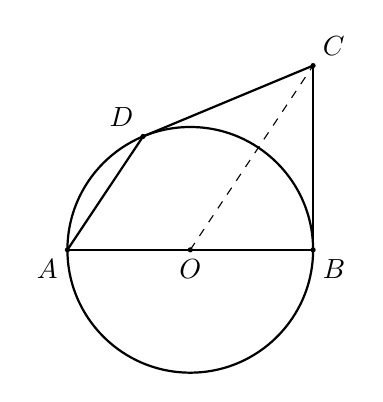
\begin{tikzpicture}[scale=0.78,>=stealth]
  \coordinate (O) at (0,0);
  \coordinate (A) at (-2,0);
  \coordinate (B) at (2,0);
  \coordinate (C) at (2,3);
  \coordinate (D) at (-0.769,1.846);
  \draw[thick] (O) circle (2);
  \draw[thick] (A)--(B);
  \draw[thick] (B)--(C);
  \draw[thick] (A)--(D);
  \draw[thick] (D)--(C);
  \draw[dashed] (O)--(C);
  \fill (O) circle (1.2pt) node[below] {$O$};
  \fill (A) circle (1.2pt) node[below left] {$A$};
  \fill (B) circle (1.2pt) node[below right] {$B$};
  \fill (C) circle (1.2pt) node[above right] {$C$};
  \fill (D) circle (1.2pt) node[above left] {$D$};
\end{tikzpicture}
\end{center}
\nopagebreak[4]
\end{question}
\begin{question}
\gkti{3}证明：

\nopagebreak[4]
\[
\frac{\sin2\alpha+1}{1+\cos2\alpha+\sin2\alpha}=\frac12\tan\alpha+\frac12.
\]

\end{question}
\begin{question}
\gkti{4}已知 $2\lg x+\lg2=\lg(x+6)$，求 $x$。

\Needspace{0.4\textheight}
\end{question}
\begin{question}
\gkti{5}某生产队要建立一个形状是直角梯形的苗圃，其两邻边借用夹角为 $135^\circ$ 的两面墙，另外两边是总长为 $30$ 米的篱笆（如图，$AD$ 和 $DC$ 为墙），问篱笆的两边各多长时，苗圃的面积最大？最大面积是多少？
\nopagebreak[4]
\begin{center}% 1977 年河北卷第 5 题：两面墙与篱笆围成的直角梯形
\begin{tikzpicture}[scale=0.78]
  \coordinate (A) at (0,0);
  \coordinate (B) at (5.2,0);
  \coordinate (C) at (5.2,2.6);
  \coordinate (D) at (2.6,2.6);
  \draw[thick] (A)--(B)--(C)--(D)--cycle;
  \draw[very thick] (A)--(D) node[midway,left] {墙};
  \draw[very thick] (D)--(C) node[midway,above] {墙};
  \node[below left] at (A) {$A$};
  \node[below right] at (B) {$B$};
  \node[above right] at (C) {$C$};
  \node[above left] at (D) {$D$};
  \node[below] at (2.6,0) {篱笆};
  \node[right] at (5.2,1.3) {篱笆};
\end{tikzpicture}
\end{center}
\nopagebreak[4]
\end{question}
\begin{question}
\gkti{6}工人师傅要用铁皮做一个上大下小的正四棱台形容器（上面开口），使其容积为 $208$ 立方米，高为 $4$ 分米，上口边长与下底面边长的比为 $5:2$，做这样的容器需要多少平方米的铁皮？（不计容器的厚度和加工余量，不要求写出已知、求解，直接求解并画图即可。）

\Needspace{0.4\textheight}
\end{question}
\begin{question}
\gkti{7}如图，$MN$ 为圆的直径，$P\text{、}C$ 为圆上两点，连 $PM\text{、}PN$，过 $C$ 作 $MN$ 的垂线与 $MN\text{、}MP$ 和 $NP$ 的延长线依次相交于 $A\text{、}B\text{、}D$，求证：

\nopagebreak[4]
\[
AC^2=AB\cdot AD.
\]
\nopagebreak[4]
\begin{center}% 1977 年河北卷第 7 题：圆内直径与外部相交线
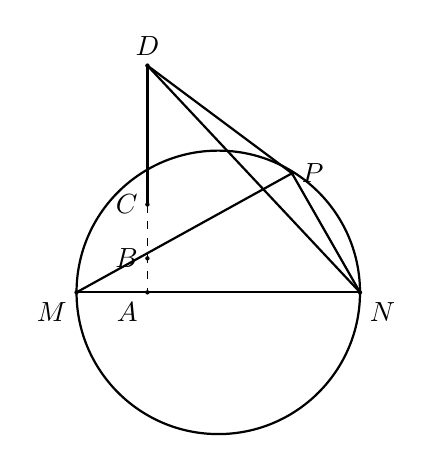
\begin{tikzpicture}[scale=0.72,>=stealth]
  \coordinate (M) at (0,0);
  \coordinate (N) at (5,0);
  \coordinate (O) at (2.5,0);
  \coordinate (P) at (3.8,2.1);
  \coordinate (C) at (1.25,1.55);
  \coordinate (D) at (1.25,4.0);
  \coordinate (A) at (1.25,0);
  \coordinate (B) at (1.25,0.6);
  \draw[thick] (M) arc (180:540:2.5);
  \draw[thick] (M)--(N);
  \draw[thick] (P)--(M) (P)--(N);
  \draw[thick] (D)--(P);
  \draw[thick] (D)--(C);
  \draw[thick] (D)--(N);
  \draw[dashed] (C)--(A);
  \fill (M) circle (1.1pt) node[below left] {$M$};
  \fill (N) circle (1.1pt) node[below right] {$N$};
  \fill (P) circle (1.1pt) node[right] {$P$};
  \fill (C) circle (1.1pt) node[left] {$C$};
  \fill (D) circle (1.1pt) node[above] {$D$};
  \fill (A) circle (1.1pt) node[below left] {$A$};
  \fill (B) circle (1.1pt) node[left] {$B$};
\end{tikzpicture}
\end{center}
\nopagebreak[4]
\end{question}
\begin{question}
\gkti{8}下列两题选做一题。

【甲】已知椭圆短轴长为 $2$，中心与抛物线 $y^2=4x$ 的顶点重合，椭圆的一个焦点恰是此抛物线的焦点，求椭圆方程及其长轴的长。

【乙】已知菱形的一对内角各为 $60^\circ$，边长为 $4$，以菱形对角线所在的直线为坐标轴建立直角坐标系，以菱形 $60^\circ$ 角的两个顶点为焦点，并且过菱形的另外两个顶点作椭圆，求椭圆方程。

\begin{gktip}
\Needspace{0.25\textheight}
\textbf{附加题}
\end{gktip}

\textbf{附加题 9．} 将函数 $f(x)=\mathrm e^x$ 展开为 $x$ 的幂级数，并求出收敛区间。（$\mathrm e=2.718$ 为自然对数的底数。）

\end{question}